\begin{appendix}
\chapter{Appendix}
\vspace{-0.2cm}
\section{Usage of the Open Sigfox Stack}
\vspace{-0.2cm}
\label{sec:renard_usage}
\subsection{How to Obtain}
\vspace{-0.2cm}
As previously mentioned, the open Sigfox stack consists of a library \texttt{librenard} and its command line frontend \texttt{renard}.
Both are open source and can be obtained from their respective GitHub repositories\footnote{\label{fn:repo_private_note}At the time of writing, these repositories are set to ``private'', which means that they are not publicly accessible. This will change once this thesis is publicly presented. Please contact the author if you want to request access.} at \url{https://github.com/Jeija/renard} and \url{https://github.com/Jeija/librenard}.
Up-to-date instructions on how to download (or ``clone'' in \texttt{git} jargon) the repositories, install dependencies and compile \texttt{renard} and \texttt{lib\-renard} can also be found on these websites.

\vspace{-0.2cm}
\subsection{Documentation}
\vspace{-0.2cm}
Both \texttt{renard} and\texttt{librenard} are extensively documented.
\texttt{librenard}'s documentation is programmatically generated using Doxygen\footnote{\url{http://www.doxygen.org/}} and Sphinx\footnote{\url{https://www.sphinx-doc.org}} and the most up-to-date version is automatically published to the \textit{Read the Docs} documentation hosting platform at \url{https://librenard.readthedocs.io}\footnote{At the time of writing, documentation on \textit{Read the Docs} is not publicly available. It can be manually compiled as described in \texttt{librenard}'s \textit{README} file though.}, whose graphical interface is shown in \Cref{fig:librenard_rtd}.

\begin{figure}[h]
	\centering
	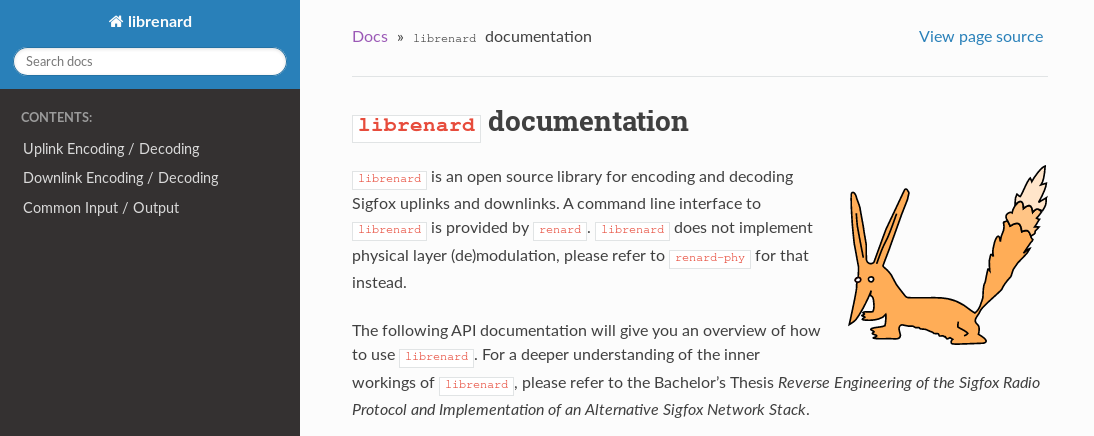
\includegraphics[width=0.7\textwidth]{fig/librenard_doc_screenshot.png}
	\caption{Screenshot of \texttt{librenard}'s programmatically generated documentation.}
	\label{fig:librenard_rtd}
\end{figure}

Given that \texttt{librenard}'s programming interface may change in future versions, detailed instructions on how to use \texttt{librenard} are omitted here.
Please refer to the online documention for current information on the usage of \texttt{librenard}.
The latest version of \texttt{renard}'s documentation on the other hand can be found in the \textit{README} file in its GitHub repository.
Again, specifics on the usage of \texttt{renard} were excluded from this thesis as they may be subject to change.

\FloatBarrier
\section{Usage of Modulation / Demodulation Scripts}
\label{sec:demodscripts}
\subsection{How to Obtain}
Open source modulation and demodulation scripts are published on GitHub\footnote{See \Cref{fn:repo_private_note}} at \url{https://github.com/Jeija/renard-phy} under the name \texttt{renard-phy}.
They currently support WAV file recordings for demodulation and the \textit{HackRF One} (shown in \Cref{fig:hackrf_sipy}) for transmission, other \gls{sdr} hardware is currently not supported.
The above-mentioned repository website also contains instructions on how to download \texttt{renard-phy} and on how to install necessary dependencies.

\begin{figure}[h]
	\centering
	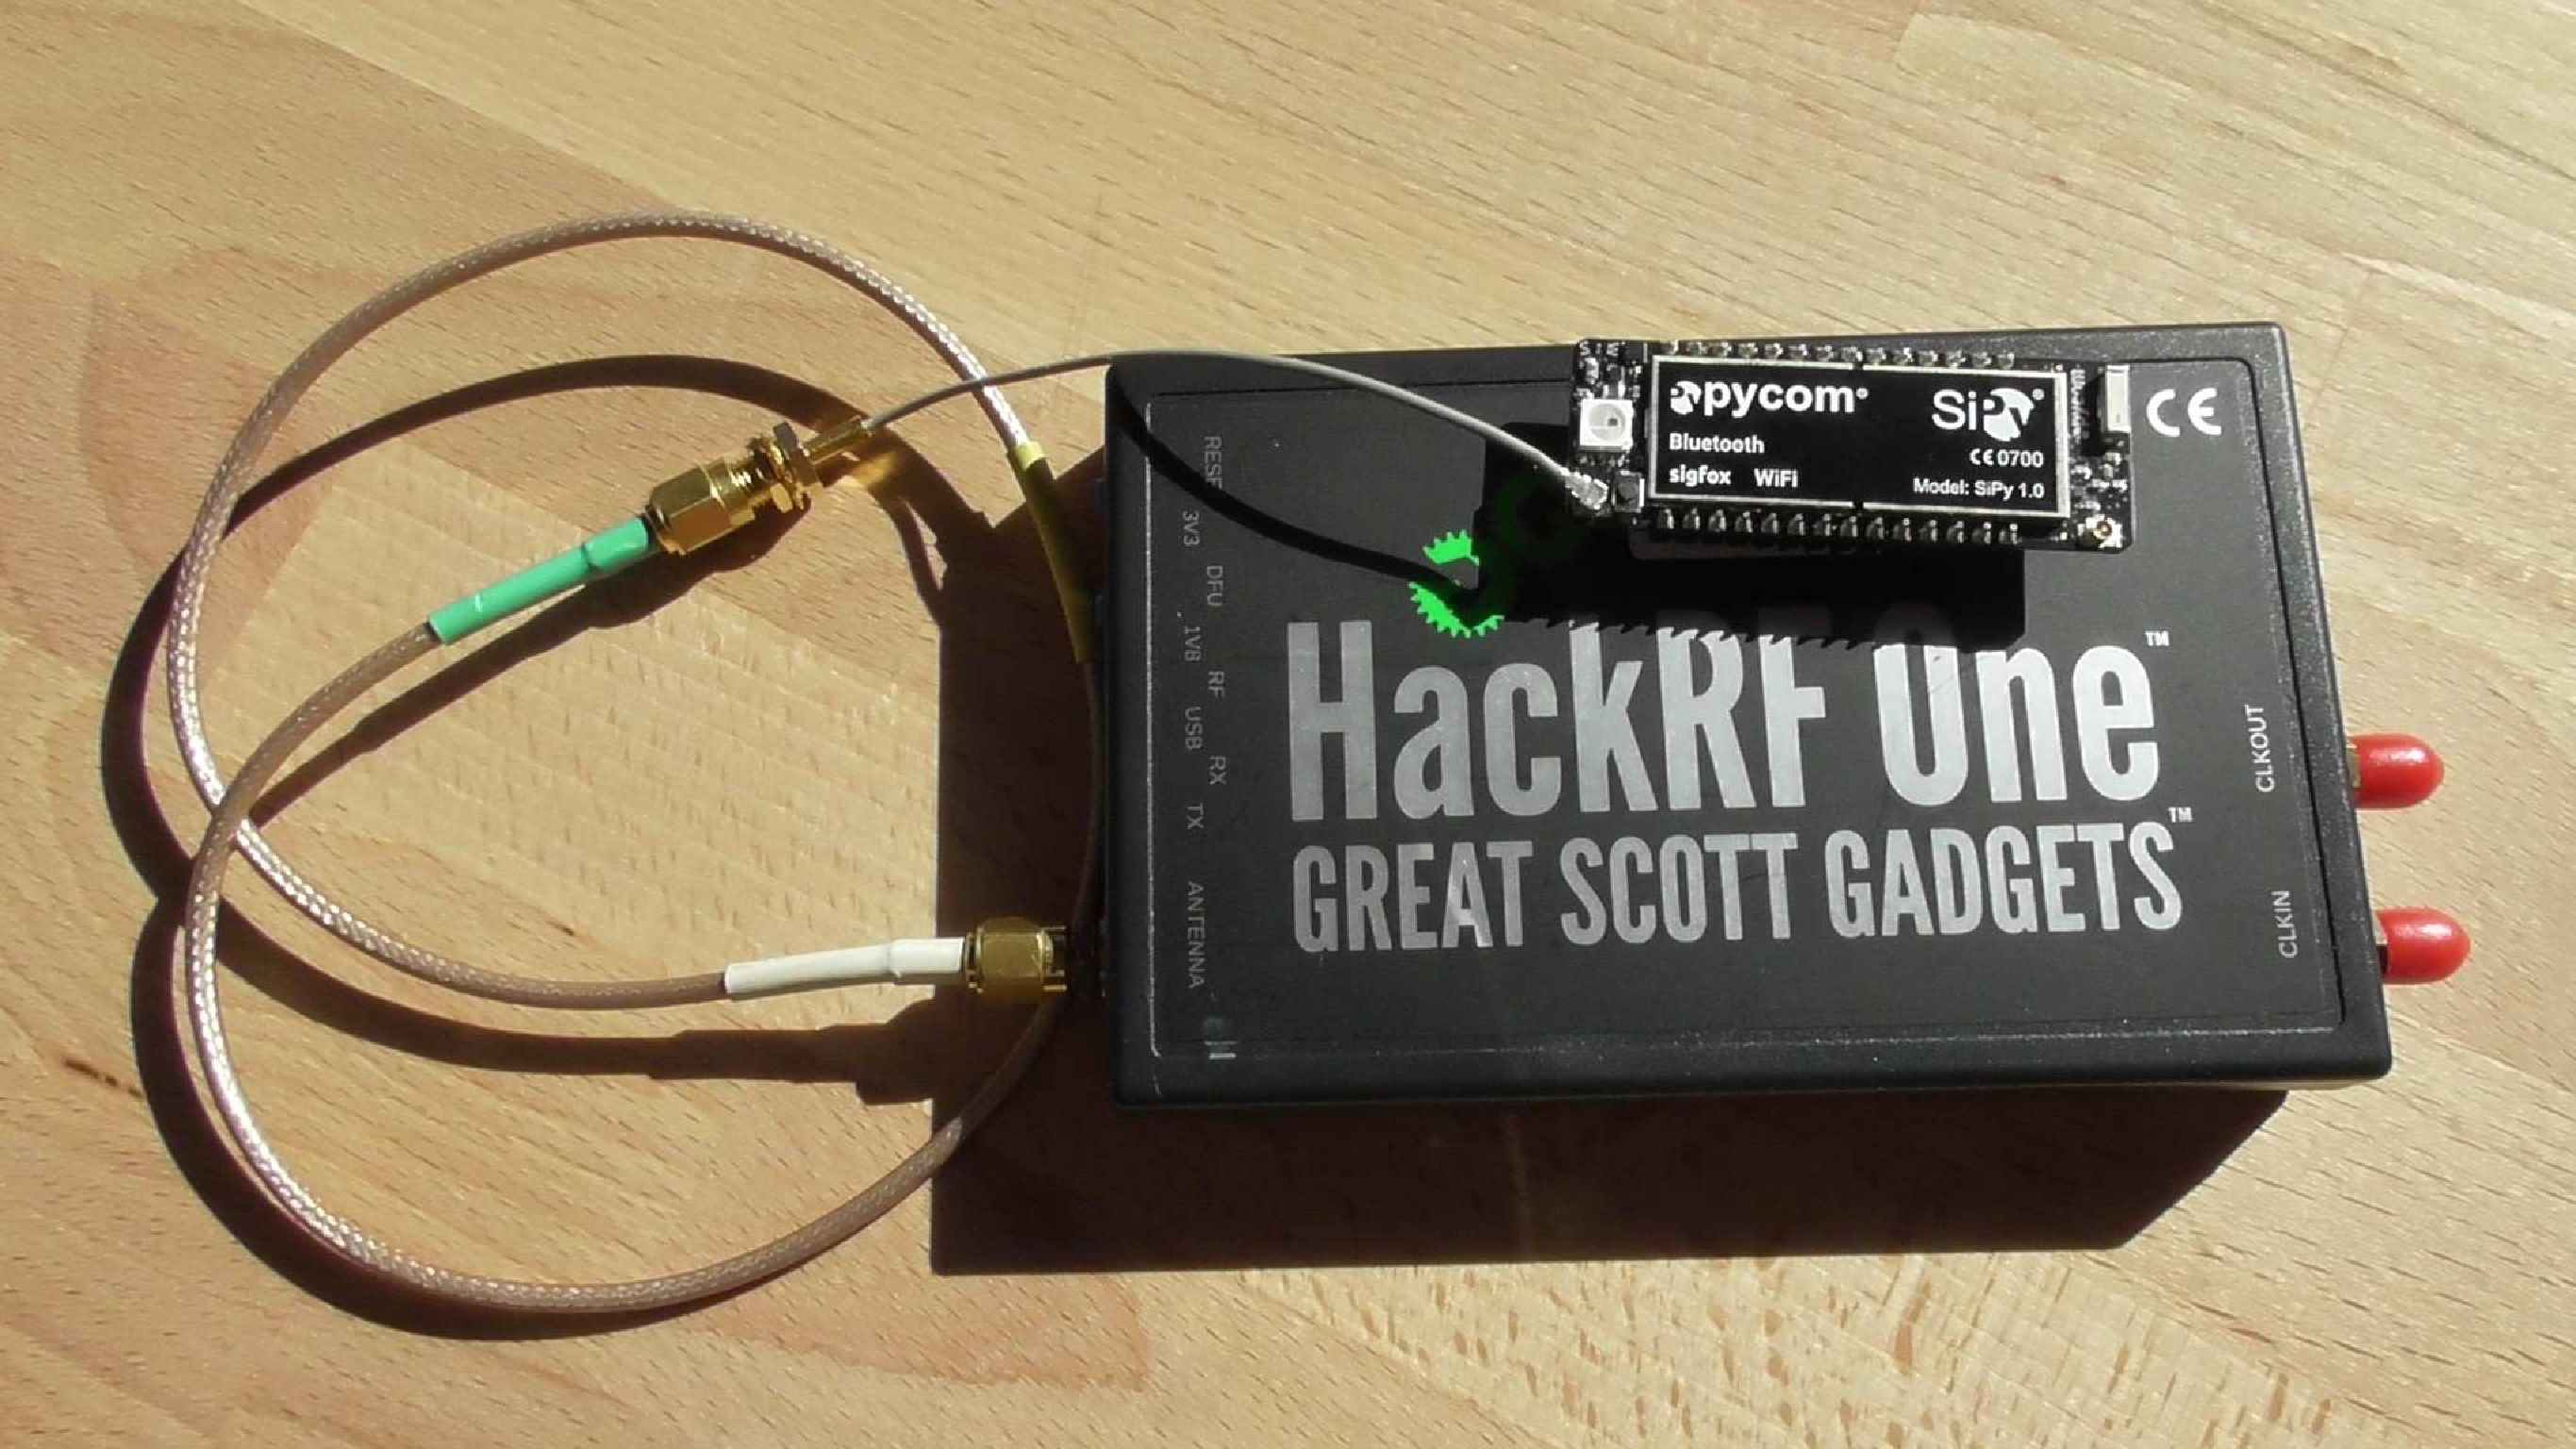
\includegraphics[width=0.5\textwidth]{fig/hackrf.png}
	\caption{\textit{Pycom SiPy} directly connected to a \textit{HackRF One}}
	\label{fig:hackrf_sipy}
\end{figure}

\subsection{Documentation}
Detailed information on how to use the latest \texttt{renard-phy} version at any given time are available in \texttt{renard-phy}'s \textit{README} file.
It also contains instructions on how to obtain sample WAV recordings of Sigfox uplinks and downlinks that can be used for testing, so that posession of suitable \gls{sdr} hardware is not required for development.
Since \texttt{renard-phy}'s interface may be subject to change in future versions, specifics on \texttt{renard-phy}'s usage are omitted from this thesis.

\section{Overview of Analysis Methods}
\label{sec:analysismethods}
\subsection{Recording Transmissions}
Using the \textit{HackRF One} and an RTL-SDR \footnote{\url{https://osmocom.org/projects/rtl-sdr/wiki}}, both uplink and downlink frames were captured with GQRX.
Tools like inspectrum \footnote{\url{https://github.com/miek/inspectrum}}, GNU Radio \footnote{\url{https://www.gnuradio.org/}}, Universal Radio Hacker \footnote{\url{https://github.com/jopohl/urh}} and Audacity \footnote{\url{https://www.audacityteam.org/}} (see also \Cref{fig:audacity}) were used to inspect the recorded WAV files.
These tools were used to form / confirm hypotheses for the used modulation schemes and as an aid in developing demodulation scripts.

\begin{figure}[h]
	\centering
	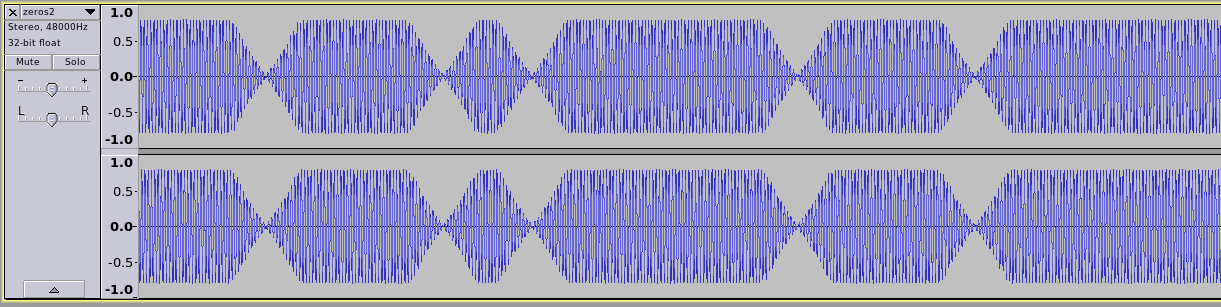
\includegraphics[width=0.8\textwidth]{fig/audacity_uplink.png}
	\caption{Excerpt of a WAV recording of an uplink visualized in Audacity, clearly showing that filtering is applied}
	\label{fig:audacity}
\end{figure}

\subsection{Online Research}
Extensive research in datasheets, patent databases, application notes or searching for binary blob symbol names on the internet can sometimes also lead to new insights.
In reverse engineering communities, this method is sometimes also jokingly known as \gls{osint}, a phrase that is otherwise mostly used in the context of intelligence agencies.
Where \gls{osint} methods have been successful in this thesis, they are noted and appropriate references to online resources are provided.

\end{appendix}
